\documentclass[aspectratio=169,10pt]{beamer}

\usepackage{amsmath,amssymb}
\usepackage{booktabs}
\usepackage{array}
\usepackage{tikz}
\usepackage{hyperref}
\usetikzlibrary{arrows.meta,positioning,shapes.geometric,calc}

\usetheme{default}

% ---------------------------------------------------------
% COLORS
% ---------------------------------------------------------
\definecolor{Navy}{RGB}{25,43,70}
\definecolor{Blue}{RGB}{48,93,150}
\definecolor{Teal}{RGB}{35,130,135}
\definecolor{LightBlue}{RGB}{237,244,251}
\definecolor{LightTeal}{RGB}{233,247,246}
\definecolor{LightOrange}{RGB}{253,244,231}
\definecolor{LightPurple}{RGB}{244,241,250}
\definecolor{DarkGray}{RGB}{60,65,70}
\definecolor{MediumGray}{RGB}{105,110,115}
\definecolor{LightGray}{RGB}{246,247,249}

% ---------------------------------------------------------
% BEAMER STYLE
% ---------------------------------------------------------
\setbeamertemplate{navigation symbols}{}
\setbeamersize{text margin left=0.55cm,text margin right=0.55cm}

\setbeamercolor{normal text}{fg=DarkGray,bg=white}
\setbeamercolor{structure}{fg=Blue}
\setbeamercolor{frametitle}{fg=white,bg=Navy}
\setbeamerfont{frametitle}{size=\large,series=\bfseries}

\setbeamertemplate{frametitle}{%
  \nointerlineskip%
  \begin{beamercolorbox}[wd=\paperwidth,ht=0.78cm,dp=0.14cm,leftskip=0.55cm]{frametitle}%
    \usebeamerfont{frametitle}\insertframetitle%
  \end{beamercolorbox}%
}

\setbeamertemplate{footline}{%
  \leavevmode%
  \hbox{%
    \begin{beamercolorbox}[wd=.78\paperwidth,ht=0.25cm,dp=0.06cm,leftskip=0.55cm]{author in head/foot}%
      \color{MediumGray}\tiny EV Charging Infrastructure Optimization%
    \end{beamercolorbox}%
    \begin{beamercolorbox}[wd=.22\paperwidth,ht=0.25cm,dp=0.06cm,rightskip=0.55cm]{author in head/foot}%
      \color{MediumGray}\tiny\hfill\insertframenumber/\inserttotalframenumber%
    \end{beamercolorbox}%
  }%
}

\setbeamertemplate{blocks}[rounded][shadow=false]
\setbeamercolor{block title}{fg=Navy,bg=LightBlue}
\setbeamercolor{block body}{fg=DarkGray,bg=LightBlue!45}

\setbeamertemplate{itemize item}{\color{Teal}\scriptsize$\bullet$}
\setbeamertemplate{itemize subitem}{\color{Teal}\scriptsize$\bullet$}

% ---------------------------------------------------------
% TIKZ STYLES
% ---------------------------------------------------------
\tikzset{
  flow/.style={
    rectangle, rounded corners=3pt,
    minimum width=2.30cm, minimum height=0.70cm,
    text width=2.30cm, align=center,
    draw=Navy, line width=0.7pt,
    fill=LightBlue, font=\scriptsize
  },
  flowteal/.style={
    rectangle, rounded corners=3pt,
    minimum width=2.30cm, minimum height=0.70cm,
    text width=2.30cm, align=center,
    draw=Teal, line width=0.7pt,
    fill=LightTeal, font=\scriptsize
  },
  floworange/.style={
    rectangle, rounded corners=3pt,
    minimum width=2.30cm, minimum height=0.70cm,
    text width=2.30cm, align=center,
    draw=Blue, line width=0.7pt,
    fill=LightOrange, font=\scriptsize
  },
  flowpurple/.style={
    rectangle, rounded corners=3pt,
    minimum width=2.30cm, minimum height=0.70cm,
    text width=2.30cm, align=center,
    draw=Navy, line width=0.7pt,
    fill=LightPurple, font=\scriptsize
  },
  model/.style={
    rectangle, rounded corners=5pt,
    minimum width=3.7cm, minimum height=1.25cm,
    text width=3.7cm, align=center,
    draw=Blue, line width=0.8pt,
    fill=LightOrange, font=\scriptsize
  },
  modelteal/.style={
    rectangle, rounded corners=5pt,
    minimum width=3.7cm, minimum height=1.25cm,
    text width=3.7cm, align=center,
    draw=Teal, line width=0.8pt,
    fill=LightTeal, font=\scriptsize
  },
  outputbox/.style={
    rectangle, rounded corners=5pt,
    minimum width=3.7cm, minimum height=0.70cm,
    text width=3.7cm, align=center,
    draw=Navy, line width=0.8pt,
    fill=LightPurple, font=\scriptsize
  },
  arr/.style={-{Stealth[length=2mm]}, line width=0.8pt, draw=DarkGray}
}

% ---------------------------------------------------------
% TITLE
% ---------------------------------------------------------
\title{Strategic Optimization of EV Charging Infrastructure}
\subtitle{Applying Operations Research to Facility Location and Resource Allocation}
\author{Team D07}
\institute{Amrita School of Artificial Intelligence\\Amrita Vishwa Vidyapeetham, Coimbatore}
\date{August 2026}

\begin{document}

% =========================================================
% 1 TITLE
% =========================================================
\begin{frame}[plain]

\vspace{0.65cm}

\begin{columns}[c]

% =========================================================
% Vertical accent line
% =========================================================
\begin{column}{0.06\textwidth}

\begin{tikzpicture}
\fill[Teal] (0,0) rectangle (0.16,5.0);
\end{tikzpicture}
\end{column}

% =========================================================
% Main content
% =========================================================
\begin{column}{0.88\textwidth}

% Title
{\fontsize{24}{29}\selectfont
\color{Navy}
\textbf{EV Charging Infrastructure Optimization}}\\[-1mm]

\vspace{0.55cm}

% Group number
{\large
\textbf{Group Number:} \color{Teal}\textbf{D07}
}

\vspace{0.35cm}

% Group members heading
{\large
\color{Navy}
\textbf{Group Members:}
}

\vspace{0.18cm}

% Members
{\normalsize
\textbf{Harshvardhan V} -- CB.SC.U4AIE23353\\[1.5mm]
\textbf{Rishi Raajha A} -- CB.SC.U4AIE23335\\[1.5mm]
\textbf{Naveen Sankar R S} -- CB.SC.U4AIE23323\\[1.5mm]
\textbf{Sakthi Pranav S} -- CB.SC.U4AIE23336
}

\end{column}

\end{columns}

\end{frame}

% =========================================================
% 2 INTRODUCTION
% =========================================================
\begin{frame}{Introduction}

\vspace{0.35cm}

\begin{itemize}

    \item The rapid global transition to Electric Vehicles (EVs) requires a massive, coordinated scale-up in charging infrastructure.

    \vspace{0.35cm}

    \item Building charging stations is expensive and resource-intensive. Current deployment is often reactive rather than strategic, leading to dense clusters in some areas and ``charging deserts'' in others.

    \vspace{0.35cm}

    \item Without careful planning, infrastructure expansion can worsen geographic and demographic inequalities.

    \vspace{0.35cm}

    \item \textbf{Significance:} By leveraging Operations Research (OR) methodologies, we aim to transform subjective infrastructure planning into a rigorous, data-driven mathematical process to ensure efficiency and fairness.

\end{itemize}

\end{frame}

% =========================================================
% 3 PROBLEM STATEMENT
% =========================================================
\begin{frame}{Problem Statement}

\vspace{0.25cm}

\begin{itemize}

    \item \textbf{Core Question:} Given a limited budget and an existing network of EV chargers, how can we expand the infrastructure to maximize both geographic coverage and regional fairness?

\end{itemize}

\vspace{0.3cm}

\begin{columns}[T]
\begin{column}{0.48\textwidth}
\begin{block}{Sub-Problem 1: The Coverage Problem}
\vspace{2mm}
Where should new high-capacity charging hubs be placed to serve the highest number of existing charging stations?
\vspace{2mm}
\end{block}
\end{column}

\begin{column}{0.48\textwidth}
\begin{block}{Sub-Problem 2: The Fairness Problem}
\vspace{2mm}
How should a fixed budget of new charging connectors be allocated across administrative regions to ensure underserved areas receive adequate infrastructure?
\vspace{2mm}
\end{block}
\end{column}
\end{columns}

\vspace{0.3cm}
\begin{itemize}
    \item Simple heuristic approaches fail to consider these strict budget constraints and fairness trade-offs simultaneously. An OR framework is essential.
\end{itemize}

\end{frame}

% =========================================================
% 4 OBJECTIVES
% =========================================================
\begin{frame}{Objectives}

\vspace{0.35cm}

\begin{itemize}

    \item To mathematically model the EV charging network expansion as a set of linear and integer programming problems.

    \vspace{0.3cm}

    \item To identify optimal locations for new hubs to maximize geographic coverage under a strict budgetary constraint.

    \vspace{0.3cm}

    \item To formulate a fairness-driven allocation strategy that maximizes the minimum connectors-per-station ratio across regions.

    \vspace{0.3cm}

    \item To systematically analyze and preprocess a massive, real-world observational dataset to derive parameters for these models.

    \vspace{0.3cm}

    \item To build an interactive, data-driven decision support dashboard that allows stakeholders to run these mathematical models in real-time.

\end{itemize}

\end{frame}

% =========================================================
% 5 DATASET OVERVIEW
% =========================================================
\begin{frame}{Dataset: Global EV Charging Stations}
\vspace{0.05cm}
\begin{columns}[T]
\begin{column}{0.54\textwidth}
{\large\color{Navy}\textbf{Dataset Overview}}
\vspace{0.15cm}
\begin{itemize}
\item Public infrastructure dataset sourced from \textbf{Kaggle} (\textit{Rishi Panchal}).
\item \textbf{Dataset Size:} Comprises \textbf{10,000 records} spanning \textbf{14 parameters/features}.
\item We are focusing on a dataset of \textbf{10,000 charging-station records} comprising \textbf{14,565 connectors}.
\item \textbf{Why this dataset?} It provides a highly realistic snapshot of infrastructure, necessary for spatial and capacity-based optimization.
\end{itemize}
\end{column}
\begin{column}{0.44\textwidth}
\begin{center}
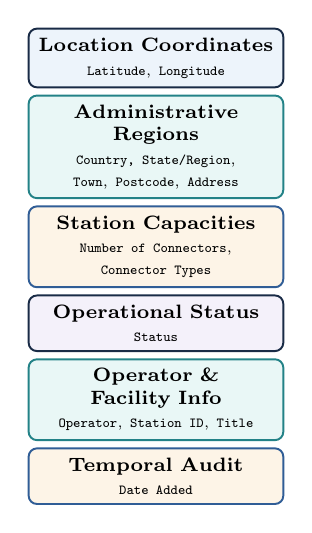
\begin{tikzpicture}[node distance=0.08cm]
\node (t) [flow, text width=3.0cm, minimum width=3.1cm] {\textbf{Location Coordinates}\\[0.2mm]\tiny\texttt{Latitude}, \texttt{Longitude}};
\node (p) [flowteal, below=of t, text width=3.0cm, minimum width=3.1cm] {\textbf{Administrative Regions}\\[0.2mm]\tiny\texttt{Country, State/Region}, \texttt{Town}, \texttt{Postcode}, \texttt{Address}};
\node (pr) [floworange, below=of p, text width=3.0cm, minimum width=3.1cm] {\textbf{Station Capacities}\\[0.2mm]\tiny\texttt{Number of Connectors}, \texttt{Connector Types}};
\node (c) [flowpurple, below=of pr, text width=3.0cm, minimum width=3.1cm] {\textbf{Operational Status}\\[0.2mm]\tiny\texttt{Status}};
\node (d) [flowteal, below=of c, text width=3.0cm, minimum width=3.1cm] {\textbf{Operator \& Facility Info}\\[0.2mm]\tiny\texttt{Operator}, \texttt{Station ID}, \texttt{Title}};
\node (e) [floworange, below=of d, text width=3.0cm, minimum width=3.1cm] {\textbf{Temporal Audit}\\[0.2mm]\tiny\texttt{Date Added}};
\end{tikzpicture}
\end{center}
\end{column}
\end{columns}
\end{frame}

% =========================================================
% 6 DATA PARAMETERS
% =========================================================
\begin{frame}{Dataset: From Raw Data to OR Parameters}
\vspace{0.1cm}
\begin{center}\scriptsize\color{MediumGray}The raw records will be transformed into the parameters required by the two optimization models.\end{center}
\vspace{0.2cm}
\begin{columns}[T]
\begin{column}{0.32\textwidth}
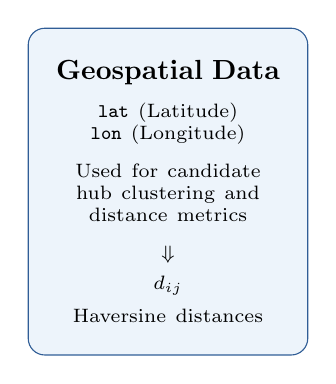
\begin{tikzpicture}
\node[rectangle,rounded corners=6pt,draw=Blue,fill=LightBlue,minimum width=3.55cm,minimum height=4.15cm,text width=3.15cm,align=center]{
\textbf{Geospatial Data}\\[2mm]
\scriptsize\texttt{lat} (Latitude)\\
\scriptsize\texttt{lon} (Longitude)\\[2mm]
Used for candidate hub clustering and distance metrics\\[2mm]
$\Downarrow$\\[1mm]
\textbf{$d_{ij}$}\\
Haversine distances};
\end{tikzpicture}
\end{column}
\begin{column}{0.32\textwidth}
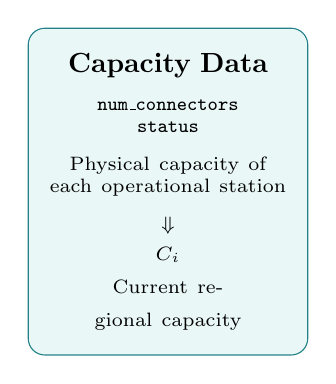
\begin{tikzpicture}
\node[rectangle,rounded corners=6pt,draw=Teal,fill=LightTeal,minimum width=3.55cm,minimum height=4.15cm,text width=3.15cm,align=center]{
\textbf{Capacity Data}\\[2mm]
\scriptsize\texttt{num\_connectors}\\
\scriptsize\texttt{status}\\[2mm]
Physical capacity of each operational station\\[2mm]
$\Downarrow$\\[1mm]
\textbf{$C_i$}\\
Current regional capacity};
\end{tikzpicture}
\end{column}
\begin{column}{0.32\textwidth}
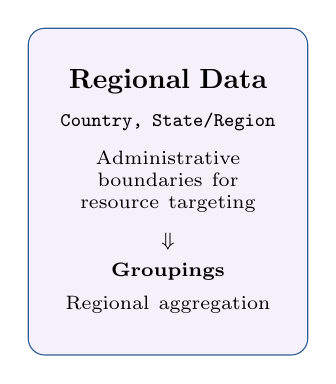
\begin{tikzpicture}
\node[rectangle,rounded corners=6pt,draw=Blue,fill=LightPurple,minimum width=3.55cm,minimum height=4.15cm,text width=3.15cm,align=center]{
\textbf{Regional Data}\\[2mm]
\scriptsize\texttt{Country, State/Region}\\[2mm]
Administrative boundaries for resource targeting\\[2mm]
$\Downarrow$\\[1mm]
\textbf{Groupings}\\
Regional aggregation};
\end{tikzpicture}
\end{column}
\end{columns}
\vspace{0.25cm}
\begin{center}\textcolor{Navy}{\textbf{Raw Data $\rightarrow$ Exploratory Data Analysis (EDA) $\rightarrow$ OR Models}}\end{center}
\end{frame}

% =========================================================
% 7 METHODOLOGY
% =========================================================
\begin{frame}{Proposed Methodology}
\vspace{0.02cm}
\begin{center}
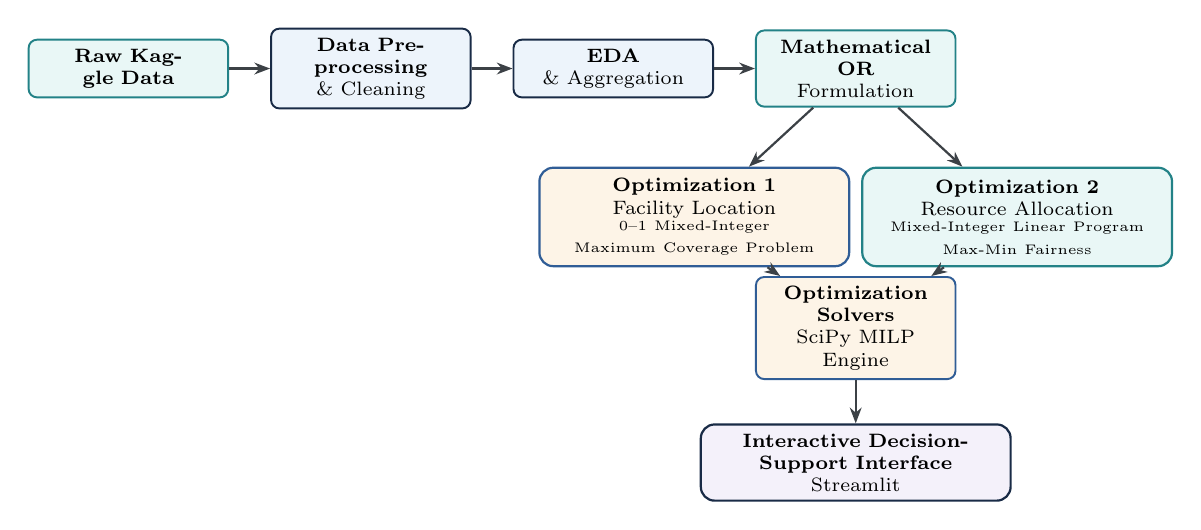
\begin{tikzpicture}[node distance=0.55cm and 0.52cm]
\node (raw) [flowteal] {\textbf{Raw Kaggle Data}};
\node (clean) [flow, right=of raw] {\textbf{Data Preprocessing}\\\& Cleaning};
\node (eda) [flow, right=of clean] {\textbf{EDA}\\\& Aggregation};
\node (param) [flowteal, right=of eda] {\textbf{Mathematical OR}\\Formulation};
\draw[arr] (raw)--(clean); \draw[arr] (clean)--(eda); \draw[arr] (eda)--(param);

\node (promo) [model, below=0.75cm of param, xshift=-2.05cm] {\textbf{Optimization 1}\\Facility Location\\\tiny 0--1 Mixed-Integer\\\tiny Maximum Coverage Problem};
\node (camp) [modelteal, below=0.75cm of param, xshift=2.05cm] {\textbf{Optimization 2}\\Resource Allocation\\\tiny Mixed-Integer Linear Program\\\tiny Max-Min Fairness};
\draw[arr] (param)--(promo); \draw[arr] (param)--(camp);

\node (solver) [floworange, below=0.75cm of $(promo)!0.5!(camp)$] {\textbf{Optimization Solvers}\\SciPy MILP Engine};
\draw[arr] (promo)--(solver); \draw[arr] (camp)--(solver);

\node (ui) [outputbox, below=0.55cm of solver] {\textbf{Interactive Decision-Support Interface}\\Streamlit};
\draw[arr] (solver)--(ui);
\end{tikzpicture}
\end{center}
\vspace{0.02cm}
\end{frame}

% =========================================================
% 8 OPT 1
% =========================================================
\begin{frame}{Optimization 1: Hub Location}
\vspace{-0.1cm}
\begin{center}\color{Blue}\textbf{Mixed-Integer Programming: Facility Location (Maximum Coverage)}\end{center}
\vspace{0.1cm}

% Top Banner: Raw Data -> OR Parameter Translation
\begin{block}{Raw Data $\rightarrow$ OR Parameters Translation}
\scriptsize
\textbf{Input Data:} Latitude and longitude of coverage stations after preprocessing $\xrightarrow{\text{Spherical K-Means}}$ $M$ Candidate Hubs ($j$).\\
\textbf{Distance Matrix:} $d_{ij} = \text{Haversine}(\text{station}_i, \text{hub}_j) \implies N_i = \{j \mid d_{ij} \le R\}$ (Hubs within radius $R$).
\end{block}

\vspace{0.1cm}
\begin{columns}[T]
\begin{column}{0.32\textwidth}
\begin{block}{Decision Variables}
\scriptsize
\textbf{$y_j \in \{0,1\}$}: Select candidate hub $j$ ($j=1\dots M$).\\[1.5mm]
\textbf{$z_i \in \{0,1\}$}: Binary coverage state of station $i$ ($i=1\dots N$).
\end{block}
\end{column}

\begin{column}{0.34\textwidth}
\begin{block}{Objective Function}
\centering
\[
\boxed{\displaystyle \max Z = \sum_{i=1}^{N} z_i}
\]
\vspace{-1mm}
\raggedright
\scriptsize Maximize total existing stations covered by at least one selected hub.
\end{block}
\end{column}

\begin{column}{0.31\textwidth}
\begin{block}{Constraints}
\scriptsize
\textbf{1. Hub Limit Constraint:}\\
$\sum_{j=1}^{M} y_j \le K$ \quad (Max $K$ hubs)\\[1.5mm]
\textbf{2. Coverage Constraint:}\\
$z_i \le \sum_{j \in N_i} y_j \quad \forall i$
\end{block}
\end{column}
\end{columns}

\vspace{0.2cm}
\begin{center}
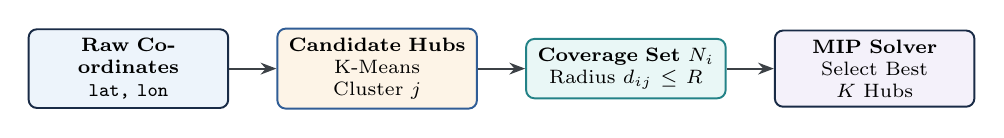
\begin{tikzpicture}[node distance=0.6cm]
\node (a) [flow] {\textbf{Raw Coordinates}\\\texttt{lat, lon}};
\node (b) [floworange, right=of a] {\textbf{Candidate Hubs}\\K-Means Cluster $j$};
\node (c) [flowteal, right=of b] {\textbf{Coverage Set $N_i$}\\Radius $d_{ij} \le R$};
\node (d) [flowpurple, right=of c] {\textbf{MIP Solver}\\Select Best $K$ Hubs};
\draw[arr](a)--(b);\draw[arr](b)--(c);\draw[arr](c)--(d);
\end{tikzpicture}
\end{center}
\end{frame}

% =========================================================
% 8 OPT 2
% =========================================================
\begin{frame}{Optimization 2: Connector Allocation}
\vspace{-0.1cm}
\begin{center}\color{Teal}\textbf{Mixed-Integer Linear Programming: Resource Allocation (Max-Min Fairness)}\end{center}
\vspace{0.1cm}

% Top Banner: Raw Data -> OR Parameter Translation
\begin{block}{Raw Data $\rightarrow$ OR Parameters Translation}
\scriptsize
\textbf{Grouping:} \texttt{Country + State/Region} $\to$ Administrative regions ($i=1\dots R$).\\
\textbf{Operational Stations ($S_i$):} Number of operational stations in region $i$.\quad
\textbf{Operational Connectors ($C_{i,\text{old}}$):} Existing operational connectors in region $i$.
\end{block}

\vspace{0.1cm}
\begin{columns}[T]
\begin{column}{0.48\textwidth}
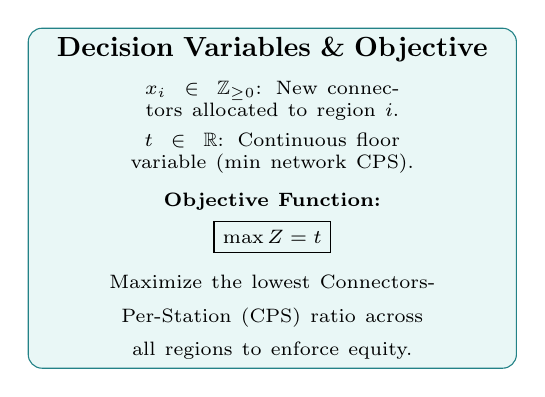
\begin{tikzpicture}
\node[rectangle,rounded corners=5pt,draw=Teal,fill=LightTeal,minimum width=6.2cm,minimum height=3.5cm,text width=5.8cm,align=center]{
\textbf{Decision Variables \& Objective}\\[2mm]
\scriptsize
\textbf{$x_i \in \mathbb{Z}_{\ge 0}$}: New connectors allocated to region $i$.\\[1mm]
\textbf{$t \in \mathbb{R}$}: Continuous floor variable (min network CPS).\\[2mm]
\textbf{Objective Function:}\\[1mm]
$\displaystyle \boxed{\max Z = t}$\\[1.5mm]
\scriptsize Maximize the lowest Connectors-Per-Station (CPS) ratio across all regions to enforce equity.
};
\end{tikzpicture}
\end{column}

\begin{column}{0.48\textwidth}
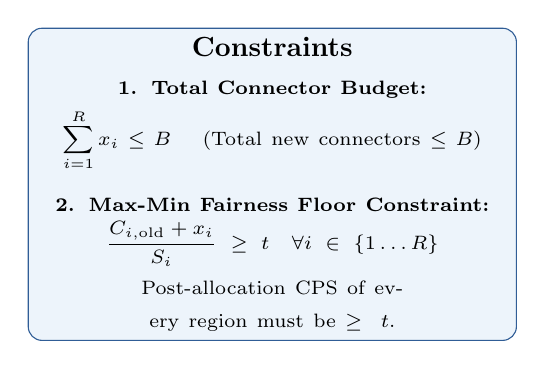
\begin{tikzpicture}
\node[rectangle,rounded corners=5pt,draw=Blue,fill=LightBlue,minimum width=6.2cm,minimum height=3.5cm,text width=5.8cm,align=center]{
\textbf{Constraints}\\[2mm]
\scriptsize
\textbf{1. Total Connector Budget:}\\[1mm]
$\displaystyle \sum_{i=1}^{R} x_i \le B$ \quad (Total new connectors $\le B$)\\[3mm]
\textbf{2. Max-Min Fairness Floor Constraint:}\\[1mm]
$\displaystyle \frac{C_{i,\text{old}} + x_i}{S_i} \ge t \quad \forall i \in \{1 \dots R\}$\\[1.5mm]
Post-allocation CPS of every region must be $\ge t$.
};
\end{tikzpicture}
\end{column}
\end{columns}

\vspace{0.2cm}
\begin{center}\textcolor{Navy}{\textbf{Raw Capacity ($C_{i,\text{old}}, S_i$) $\rightarrow$ Max-Min Allocation ($x_i$) $\rightarrow$ Network Equity ($t$)}}\end{center}
\end{frame}

% =========================================================
% 10 TOOLS
% =========================================================
\begin{frame}{Tools \& Technologies}
\vspace{0.25cm}
\begin{center}
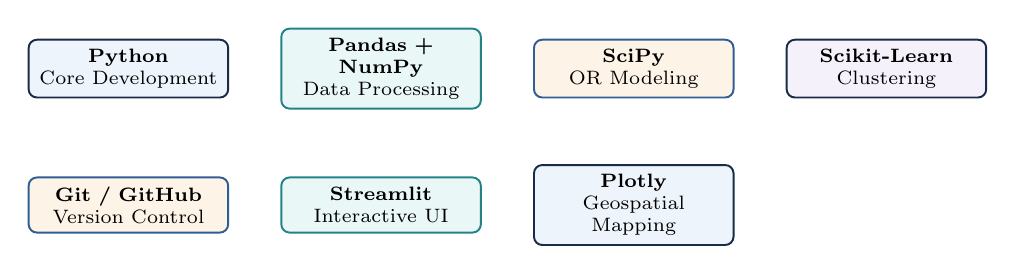
\begin{tikzpicture}[node distance=0.65cm]
\node (p) [flow] {\textbf{Python}\\Core Development};
\node (d) [flowteal, right=of p] {\textbf{Pandas + NumPy}\\Data Processing};
\node (l) [floworange, right=of d] {\textbf{SciPy}\\OR Modeling};
\node (c) [flowpurple, right=of l] {\textbf{Scikit-Learn}\\Clustering};
\node (s) [flowteal, below=0.85cm of d] {\textbf{Streamlit}\\Interactive UI};
\node (v) [flow, right=of s] {\textbf{Plotly}\\Geospatial Mapping};
\node (q) [floworange, left=of s] {\textbf{Git / GitHub}\\Version Control};
\end{tikzpicture}
\end{center}
\vspace{0.55cm}
\begin{center}

\begin{tikzpicture}
\node[rectangle,rounded corners=5pt,draw=Navy,fill=LightGray,minimum width=10.5cm,minimum height=0.65cm,text width=10.5cm,align=center]{\textbf{Data Processing $\rightarrow$ OR Modeling $\rightarrow$ Solver Optimization $\rightarrow$ Web Dashboard}};
\end{tikzpicture}
\end{center}
\vspace{0.35cm}
\end{frame}

% =========================================================
% 11. CONCLUSION
% =========================================================
\begin{frame}{Conclusion \& Next Steps}

\vspace{0.15cm}

\begin{itemize}

    \item \textbf{Summary:} The proposed framework applies rigorous Operations Research to strategic EV charging expansion, prioritizing both coverage efficiency and geographic fairness.

    \vspace{0.2cm}

    \item \textbf{Current Status:} The Kaggle dataset has been identified, and the proposed MIP/MILP formulations have been designed for the two optimization objectives.

    \vspace{0.2cm}

    \item \textbf{Next Steps:}
    \begin{itemize}
        \item Perform data preprocessing and EDA
        \item Extract parameters for both optimization models
        \item Implement and validate the optimization models using SciPy
        \item Perform sensitivity analysis for budget and coverage radius
        \item Develop the Streamlit decision-support interface
        \item Generate deployment recommendations
    \end{itemize}

\end{itemize}

\end{frame}

\end{document}
